\section{Methodology}

\subsection{Task Setup}

Samples are grouped as Conflict, Ambiguous, or Aligned.
The main experiments focus on Conflict and Aligned samples.
For each protocol, we construct \(M_1\), \(M_2\), and \(M_{12}\) conditions.

\begin{figure}[t]
  \centering
  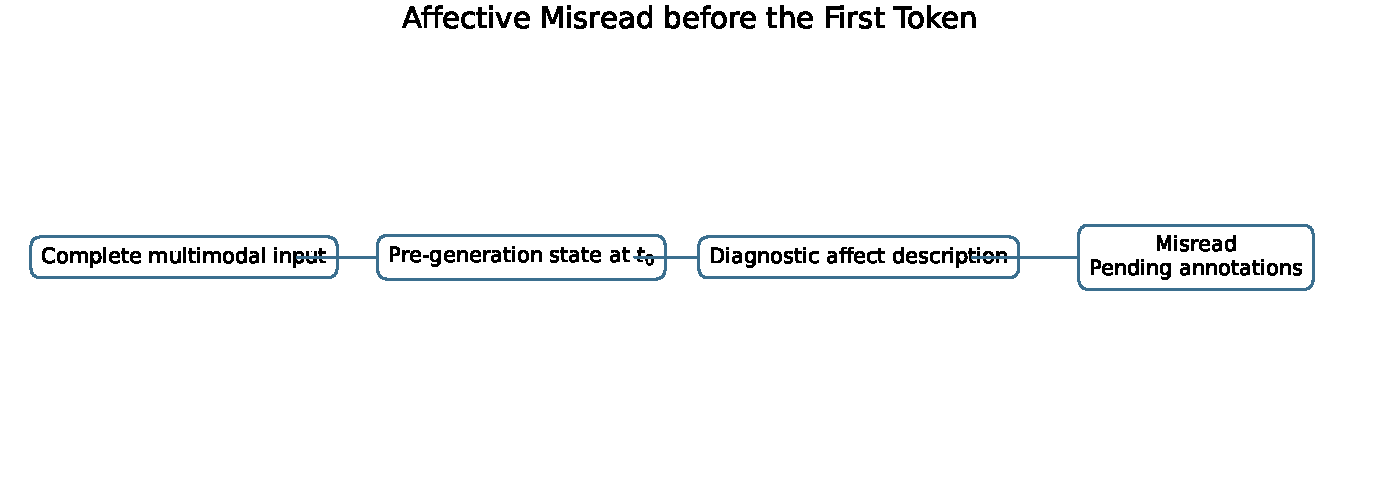
\includegraphics[width=\linewidth]{figures/generated/fig01_problem_protocol.pdf}
  \caption{Affective Misread before the first token.}
  \label{fig:problem-protocol}
\end{figure}

\subsection{Pre-generation State Extraction at \(t_0\)}

\(t_0\) is the last conditioning state before the first generated token.
The extraction uses prefill hidden states and can reuse prompt-side computation when supported.

\subsection{Pre-generation Trajectory Representation}

The state object is a full-layer prefill trajectory rather than a single hidden-state point.
The trajectory encoder maps this object into a manifold-aware representation space.

\begin{figure}[t]
  \centering
  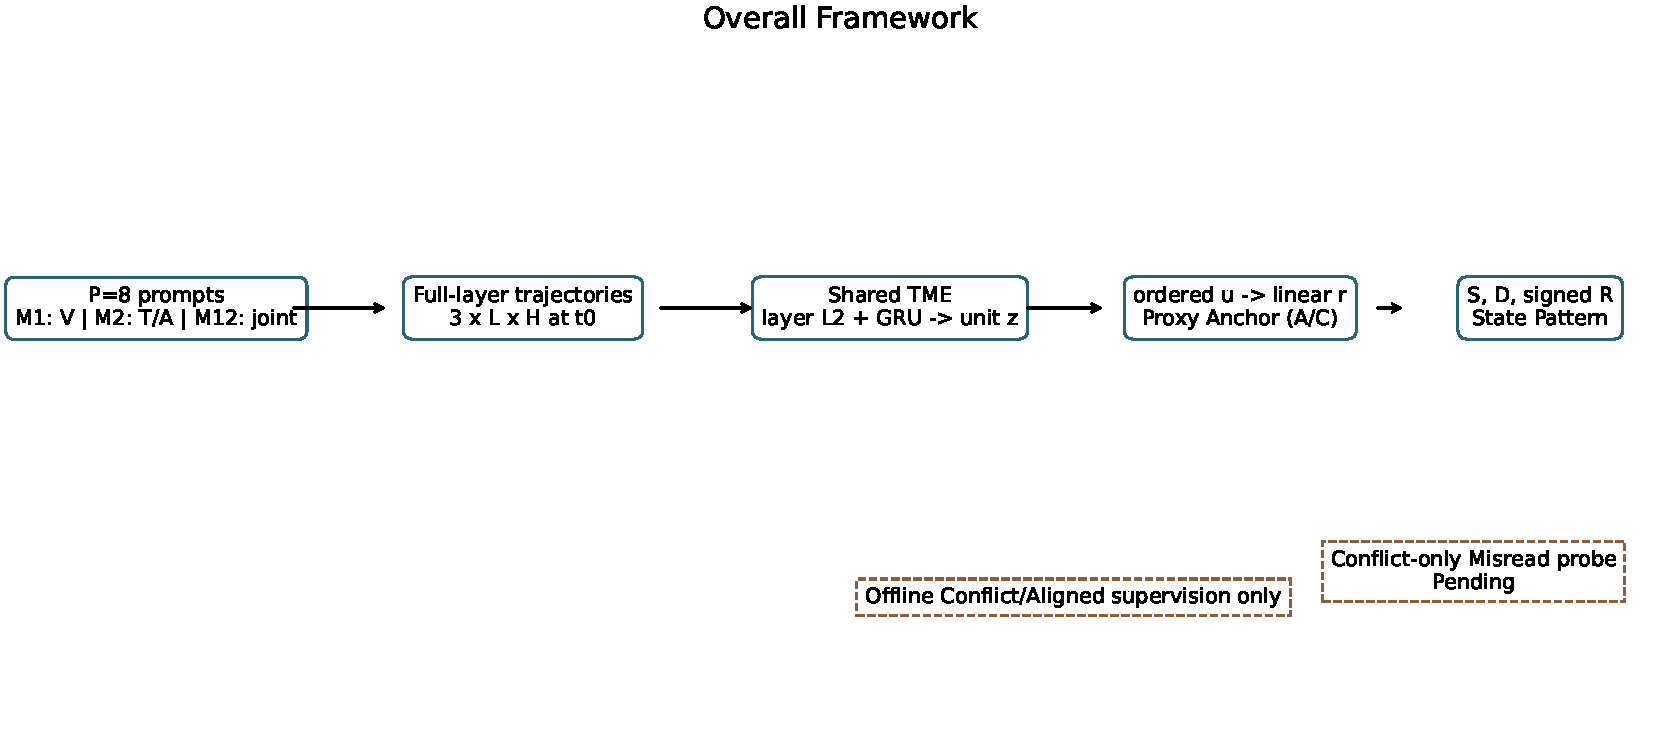
\includegraphics[width=\linewidth]{figures/generated/fig02_representation_pipeline.pdf}
  \caption{Overall framework with offline A/C supervision and the reserved Misread probe.}
  \label{fig:framework}
\end{figure}

\subsection{State Measures: \(S\), \(D\), and \(R\)}

\(S\) measures template sensitivity.
When \(S\) is large, the model may be confused or not confident.
\(D\) measures split strength.
When \(D\) is large, the input contains strong multimodal conflict.
\(R\) measures Joint Lean.
When \(R\) is large, the joint input makes the model lean toward one modality and may ignore important cues from the other.

\begin{figure}[t]
  \centering
  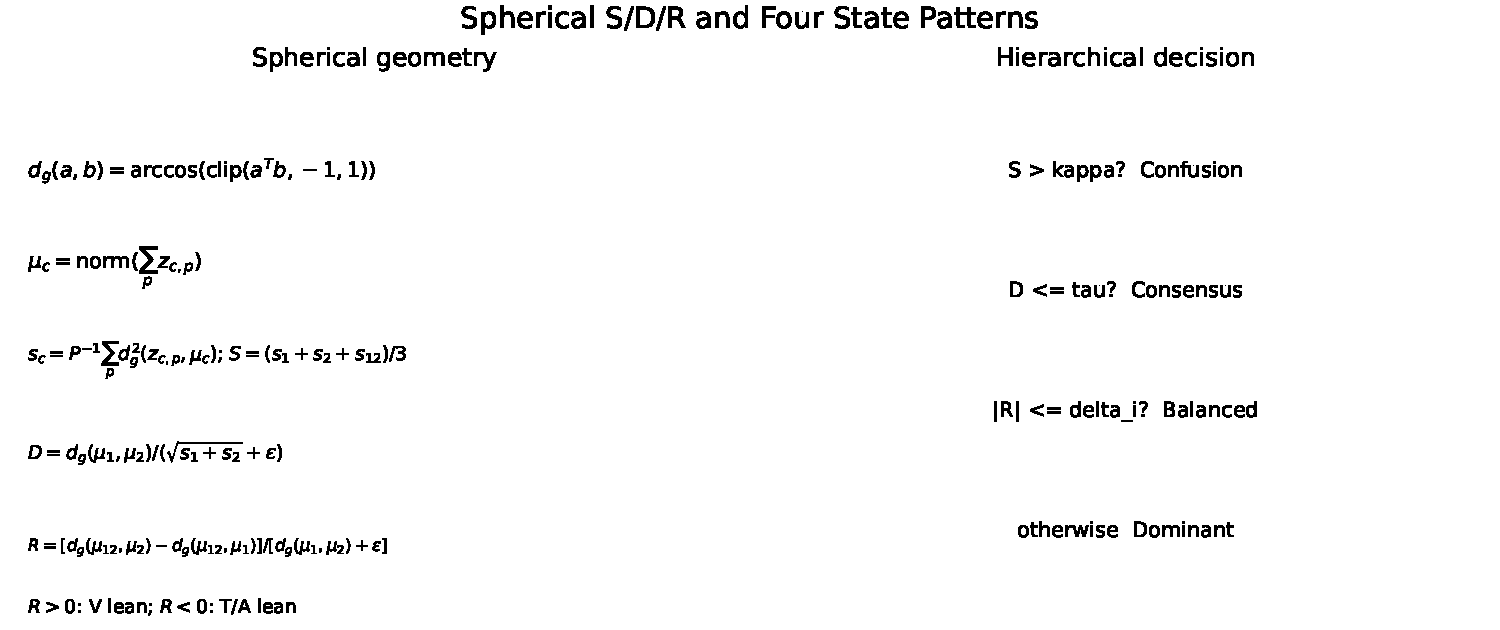
\includegraphics[width=\linewidth]{figures/generated/fig03_spherical_sdr.pdf}
  \caption{Exact spherical S/D/R definitions and hierarchical four-pattern assignment.}
  \label{fig:sdr-method}
\end{figure}

\subsection{Four State Patterns and State-guided Response}

The four patterns are Confusion, Consensus, Balanced, and Dominant.
The same state labels can be used to route a lightweight response policy in Stage 2.
